\section{The discovery of the top quark \cite{top-quark}}
After the discovery of the $b$-quark at Fermilab in 1977, the search for the $t$ quark started. It was the last missing particle to confirm the six-quark model, which is the foundation of the CKM matrix. Numerous experiments at $e^+e^-$ colliders and the SppS were just able to set lower limits for the top quark mass. It was finally discovered at the Tevatron in 1995.
\subsection{Theoretical predictions}
The top quark, with a mass of $m_t=(173.0\pm0.4)\;\si{\GeV}$, is the heaviest particle of the Standard Model. It has a charge of $\frac{2}{3}e$ and a very short mean lifetime of $\tau = 0.5\cdot 10^{-24}\;\si{\second}$. The lifetime is so short that the $t$ quark mainly decays into a $W$ boson and a $b$ quark ($V_{tb}= 1.019 \pm 0.025$), before hadronization can occur. This maximal transition probability is also the reason that single top quark production always occurs with a $b$ quark or a $W$ boson. The pair production of top quarks is always associated with gluons. Due to the short lifetime the information about the spin correlation of the $t\bar{t}$ pair persists and is preserved in the angular distribution of the decay products. In general the $t$ quark can decay via a dileptonic channel, a semi-leptonic channel or a hadronic channel, whereby the dileptonic channel is the cleanest event channel.
The high mass of the top quark is a result of the Yukawa coupling of $Y_t \approx 1$.
For this reason the Higgs boson prefers to couple to the $t$ quark. Under the assumption that BSM physics in the electroweak sector is above the SM energy scale, it couples highly to mass and therefore the top quark, as the heaviest participant should be sensitive to it.\\
It was possible to predict lower limits for the top quark mass with lepton colliders, since top quark loops are corrections to the weak boson masses. The loop corrections depend on the mass of the circulating particle. Therefore it was possible to extract predictions for the $t$ quark mass from electroweak precision measurements.

\begin{wrapfigure}{l}{0.2\textwidth}
    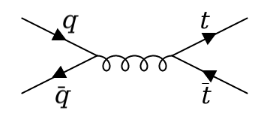
\includegraphics[width=0.18\textwidth]{graphics/tt.png}
    \caption{ $t\bar{t}$ production via $q\bar{q}$ annihilation. \cite{top-quark}}
  \end{wrapfigure}
  \FloatBarrier
For hadron colliders the production process of top quarks highly depends on the center of mass energy. Parton distribution functions (PDF) $f_i(x_i, \mu_F^2)$ describe how large the probability is to observe a specific parton $i$ with the momentum fraction $x_i$. $\mu_F^2$ is the factorization scale and corresponds to the center of mass energy. PDFs are the results of measurements and cannot be calculated with pertubative QCD. With increasing energy a proton contains a continously growing amount of $q\bar{q}$ pairs, the sea quarks, due to quantum fluctuations and after a certain point is dominated by gluons. For the energies of the Tevatron are the quark distribution functions much larger than that of the gluon. This is the reason why \SI{90}{\percent} of the events occur due to quark-antiquark annihilation. While for the LHC \SI{90}{\percent} of the events occur due to gluon fusion.
\subsection*{Measurements}
The Tevatron was part of Fermilab's accelerator chain and was a hadron collider. The experiments CDF and D\O were placed at the two collision points. Besides the top quark, the bottom quark and the tau neutrino were discovered at the Tevatron. The Tevatran had a circumference of \SI{6.3}{\kilo\meter} and accelerated protons up to nearly \SI{1}{\TeV}. In 1995, the year of the top quark discovery it was operated with a center of mass energy of $\sqrt{s}=\SI{1.8}{\TeV}$.
\subsection{The CDF Experiment}
The CDF experiment contained a magnetic spectrometer surrounded by calorimeters and muon chambers. The Silicon vertex detector was used to reconstruct tracks of charged particles. The central outer tracker was a gas filled chamber to determine the particle momenta. Both parts were surrounded by a superconducting solenoid. Outside of the magnet the electromagnetic calorimeter was located, followed by the hadronic calorimeter and the most outer part was the muon detector. It was used to measure muon tracks via position and time measurements.\\
The discovery channel of the CDF experiment was $t\bar{t} \rightarrow WbW\bar{b}$, which then either decays into two opposite charged leptons and two $b$ jets or semiletonically in one lepton and at least four jets. Therefore they required an isolated lepton with $p_{\text{t}}\geq \SI{20}{\GeV}$ and at least one $b$-tagged jet. They also removed dilepton events with an invariant mass between 75 and \SI{105}{\GeV} to exclude the pole of the $Z$ boson.
In 1995, they reached a luminosity of $\mathcal{L} = \SI{67}{\pico\barn}^{-1}$, which allowed for the discovery of the top quark.

\begin{wrapfigure}{l}{0.35\textwidth}
    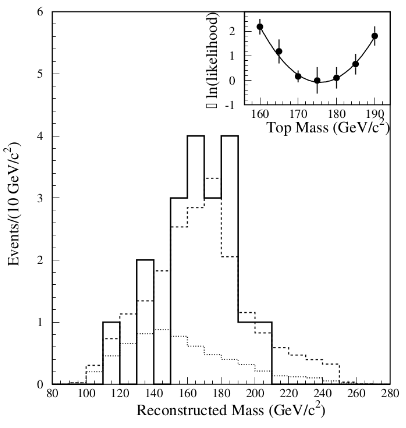
\includegraphics[width=0.33\textwidth]{graphics/CDF.png}
    \caption{Invaraint mass distribution measured with the CDF experiment to determine the top quark mass.\cite{top-quark}}
		\label{fig:CDF}
  \end{wrapfigure}
  \FloatBarrier
The collaboration considered several backgrounds for example hadrons misidentified as leptons or the production of $WW$ or $b\bar{b}$ events. They used two different taggers to reduce the background in the semileptonic decays. The secondary vertex algorithm tagged an event, if it finds a secondary vertex belonging to a $b$ jet. The soft lepton tagger searched for additional leptons of semileptonic decays of $b$ jets. The tagging reduced the number of events per amount of jets to be much closer to the expected number of background tags.\\
Figure \ref{fig:CDF} shows the reconstructed mass distribution for b-tagged measurements with more than 4 jets and the performed likelihood fit to determine the top quark mass. The dotted line shows the background (BG) shape and the dashed line the sum of $t\bar{t}$ + BG Monte Carlo events.
The best fit mass, after studies of the systematic uncertainties is:
$m_{t} = 176 \pm 18 \;\si{\GeV} $.
\subsection{The D\O Experiment}
At the D\O \;experiment a luminosity of $\mathcal{L}$ 44-56 $pb^{-1}$ was reached. For the analysis they defined the variable $H_t$ as either the scalar sum of transverse energies $E_T$ of jets for a single lepton and $\mu\mu$ + jets, or of the leading electron and jets for $e\mu$ + jets or $ee$ + jets events.
They considered different backgrounds for the dilepton channel: Z and Drell-Yan lepton pairs, the production of the vector boson pairs $WW$ or $WZ$, or the heavy flavour production $b\bar{b}$ and $c\bar{c}$. The last considered background was due to jets misidentified as leptons. The variable $H_t$ was used as a discriminator between background and signal.
They also observed a statistically significant excess of events and reconstructed the top quark mass to be $m_{t} = 199 \pm 42 \;\si{\GeV} $.

\subsection*{Outlook}
In the past years the ATLAS and CMS collaborations have carried out high precision measurements of the top quark mass with significantly reduced uncertainties. This is possible since the higher center of mass energy of the LHC allows to collect more data and therefore accesses higher statistics. The goal of high precision measurements is to reach a higher sensitivity for possible BSM physics. Other measurements that are carried out are for example the measurement of the spin correlation or the mass asymmetry of $t\bar{t}$ pairs. The latter gives the possibility to measure the $CPT$ invariance.
